\documentclass[a4paper,fleqn]{article} %Options in documentclass should be set to a4paper and fleqn.
\usepackage{times}
\usepackage{psfrag}
 \usepackage{pstricks,auto-pst-pdf}
\usepackage{pstool}
\usepackage{natbib} %The three packages modsim, times and natbib are required.
\usepackage{amsmath, amssymb, amsthm} %Also recommend the standard AMS LaTeX maths packages.

\begin{figure}[htb]
		\begin{psfrags}%
			\psfragscanon%
			%
			% text strings:
			\psfrag{s03}[t][t][2.0]{\color[rgb]{0,0,0}\setlength{\tabcolsep}{0pt}\begin{tabular}{c}$t$(s)\end{tabular}}%
			\psfrag{s04}[b][b][2.0]{\color[rgb]{0,0,0}\setlength{\tabcolsep}{0pt}\begin{tabular}{c}$h$(cm)\end{tabular}}%
			%
			% xticklabels:
			\psfrag{x01}[t][t][1.5]{50}%
			\psfrag{x02}[t][t][1.5]{51}%
			\psfrag{x03}[t][t][1.5]{52}%
			\psfrag{x04}[t][t][1.5]{53}%
			\psfrag{x05}[t][t][1.5]{54}%
			\psfrag{x06}[t][t][1.5]{55}%
			\psfrag{x07}[t][t][1.5]{56}%
			\psfrag{x08}[t][t][1.5]{57}%
			\psfrag{x09}[t][t][1.5]{58}%
			%
			% yticklabels:
			\psfrag{v01}[r][r][1.5]{-2}%
			\psfrag{v02}[r][r][1.5]{-1}%
			\psfrag{v03}[r][r][1.5]{0}%
			\psfrag{v04}[r][r][1.5]{1}%
			\psfrag{v05}[r][r][1.5]{2}%
			\psfrag{v06}[r][r][1.5]{3}%
			% Figure:
		{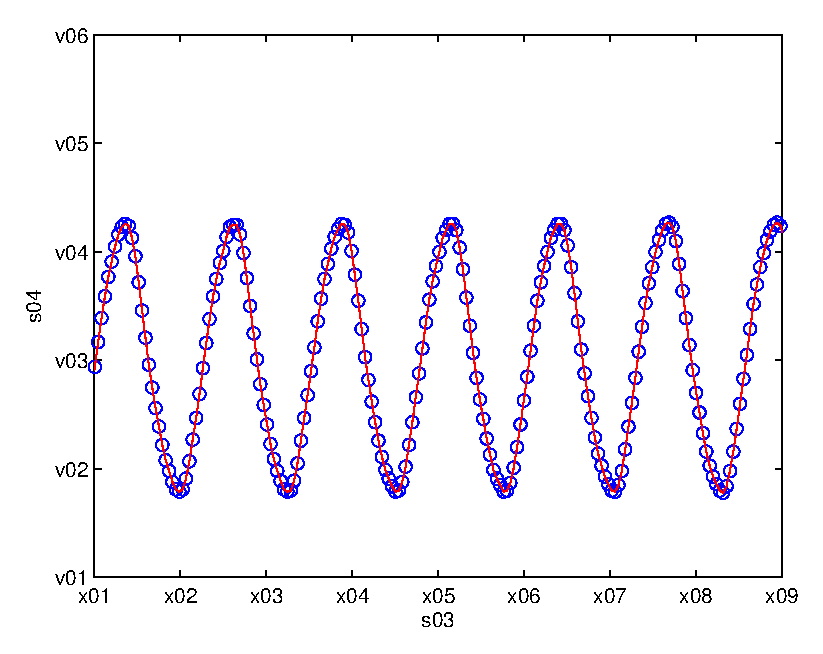
\includegraphics{Beji-1994-SH-WG1.eps}}%
		\end{psfrags}
\end{document}
